\section{Super Smash Bros. Melee}

\begin{figure}[htbp]
\begin{center}
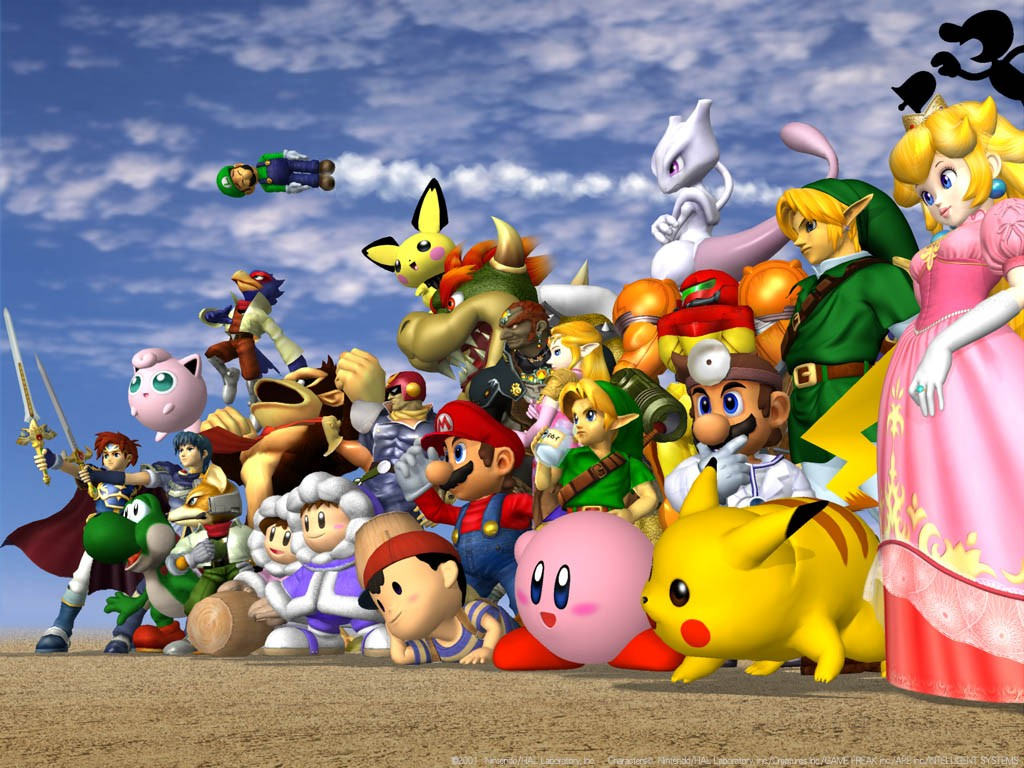
\includegraphics[width=.50\textwidth]{./imagenes/SuperSmashBrosMelee.jpg}
\caption{Super Smash Bros. Melee}
\label{Super Smash Bros. Melee}
\end{center}
\end{figure}
Super Smash Bros. Melee trata de un juego de lucha en dos dimensiones con gráficos en 3D protagonizado por 26 estrellas de Nintendo (Figura \ref{Super Smash Bros. Melee} ) de todos los tiempos. Se trata del juego más vendido de GameCube, con unas ventas superiores a 6 millones de copias en todo el mundo.

\subsubsection{¿Por qué es uno de mis juegos favoritos?}
\begin{itemize}
\item[Danny Ponce] Super Smash Bros. Melee es demasiado entretenido por su variedad en el modo de juego para un solo jugador que son cuatro: Regular Match, Event Match, Stadium, Training y para multijugador son tres: Melee, Tournament Melee y Special Melee. Este juego se deben desbloquear 11 estrellas del Nintendo, Escenarios y Trofeos jugando en cualquiera de los modos. Para mi, El modo más entretenido es Melee que puede jugar hasta 4 personas. Si hay menos de Cuatro personas para jugar, se puede seleccionar luchadores controlados por la CPU en niveles de dificultad del 1 al 9. Se pueden configurar las reglas del juego para luchar en equipos o individual y luchas por tiempo o con un número de vidas prefijado, con diferentes condiciones de victoria, como un sistema de monedas por el que con cada golpe un luchador suelta monedas y gana quien más recoge. También se puede escoger la frecuencia con la que aparecerán ítems en el escenario, desactivar algunos o todos.Una vez listos los jugadores, aparece la pantalla de selección de escenario, pudiendo elegirlo manualmente entre los desbloqueados o permitir a la consola seleccionarlo aleatoriamente.
\end{itemize}